\documentclass[11pt]{article}

\usepackage{filecontents}
\begin{filecontents}{\jobname.bib}
@article{heath2014fossilized,
  title={The fossilized birth--death process for coherent calibration of divergence-time estimates},
  author={Heath, Tracy A and Huelsenbeck, John P and Stadler, Tanja},
  journal={Proceedings of the National Academy of Sciences},
  volume={111},
  number={29},
  pages={E2957--E2966},
  year={2014},
  publisher={National Acad Sciences}
}
@article{ronquist2012mrbayes,
  title={MrBayes 3.2: efficient Bayesian phylogenetic inference and model choice across a large model space},
  author={Ronquist, Fredrik and Teslenko, Maxim and van der Mark, Paul and Ayres, Daniel L and Darling, Aaron and H{\"o}hna, Sebastian and Larget, Bret and Liu, Liang and Suchard, Marc A and Huelsenbeck, John P},
  journal={Systematic biology},
  volume={61},
  number={3},
  pages={539--542},
  year={2012},
  publisher={Oxford University Press}
}
@article{bouckaert2014beast,
  title={BEAST 2: a software platform for Bayesian evolutionary analysis},
  author={Bouckaert, Remco and Heled, Joseph and K{\"u}hnert, Denise and Vaughan, Tim and Wu, Chieh-Hsi and Xie, Dong and Suchard, Marc A and Rambaut, Andrew and Drummond, Alexei J},
  journal={PLoS Comput Biol},
  volume={10},
  number={4},
  pages={e1003537},
  year={2014},
  publisher={Public Library of Science}
}
@article{sanderson2003r8s,
  title={r8s: inferring absolute rates of molecular evolution and divergence times in the absence of a molecular clock},
  author={Sanderson, Michael J},
  journal={Bioinformatics},
  volume={19},
  number={2},
  pages={301--302},
  year={2003},
  publisher={Oxford Univ Press}
}
@article{heath2012hierarchical,
  title={A hierarchical Bayesian model for calibrating estimates of species divergence times},
  author={Heath, Tracy A},
  journal={Systematic biology},
  pages={sys032},
  year={2012},
  publisher={Oxford University Press}
}
@article{felsenstein1981evolutionary,
  title={Evolutionary trees from DNA sequences: a maximum likelihood approach},
  author={Felsenstein, Joseph},
  journal={Journal of molecular evolution},
  volume={17},
  number={6},
  pages={368--376},
  year={1981},
  publisher={Springer}
}
@article{kimura1980simple,
  title={A simple method for estimating evolutionary rates of base substitutions through comparative studies of nucleotide sequences},
  author={Kimura, Motoo},
  journal={Journal of molecular evolution},
  volume={16},
  number={2},
  pages={111--120},
  year={1980},
  publisher={Springer}
}
@article{hasegawa1985dating,
  title={Dating of the human-ape splitting by a molecular clock of mitochondrial DNA},
  author={Hasegawa, Masami and Kishino, Hirohisa and Yano, Taka-aki},
  journal={Journal of molecular evolution},
  volume={22},
  number={2},
  pages={160--174},
  year={1985},
  publisher={Springer}
}
@article{jukes1969evolution,
  title={Evolution of protein molecules},
  author={Jukes, Thomas H and Cantor, Charles R},
  journal={Mammalian protein metabolism},
  volume={3},
  pages={21--132},
  year={1969},
  publisher={New York}
}
@article{stamatakis2005raxml,
  title={RAxML-III: a fast program for maximum likelihood-based inference of large phylogenetic trees},
  author={Stamatakis, Alexandros and Ludwig, Thomas and Meier, Harald},
  journal={Bioinformatics},
  volume={21},
  number={4},
  pages={456--463},
  year={2005},
  publisher={Oxford Univ Press}
}
@article{huelsenbeck2004bayesian,
  title={Bayesian phylogenetic model selection using reversible jump Markov chain Monte Carlo},
  author={Huelsenbeck, John P and Larget, Bret and Alfaro, Michael E},
  journal={Molecular Biology and Evolution},
  volume={21},
  number={6},
  pages={1123--1133},
  year={2004},
  publisher={SMBE}
}
@article{guindon2010new,
  title={New algorithms and methods to estimate maximum-likelihood phylogenies: assessing the performance of PhyML 3.0},
  author={Guindon, St{\'e}phane and Dufayard, Jean-Fran{\c{c}}ois and Lefort, Vincent and Anisimova, Maria and Hordijk, Wim and Gascuel, Olivier},
  journal={Systematic biology},
  volume={59},
  number={3},
  pages={307--321},
  year={2010},
  publisher={Oxford University Press}
}
@article{sneath1957application,
  title={The application of computers to taxonomy},
  author={Sneath, Peter HA},
  journal={Journal of general microbiology},
  volume={17},
  number={1},
  pages={201--226},
  year={1957},
  publisher={Soc General Microbiol}
}
@article{darriba2012jmodeltest,
  title={jModelTest 2: more models, new heuristics and parallel computing},
  author={Darriba, Diego and Taboada, Guillermo L and Doallo, Ram{\'o}n and Posada, David},
  journal={Nature methods},
  volume={9},
  number={8},
  pages={772--772},
  year={2012},
  publisher={Nature Publishing Group}
}
\end{filecontents}

\usepackage{natbib}
\usepackage{adjustbox}
\usepackage{amsmath}
\usepackage[font=footnotesize]{caption}
\usepackage[dvipsnames]{xcolor}
\usepackage{geometry}
  \geometry{margin=1in}
\usepackage{framed}
\usepackage[breaklinks]{hyperref}
\usepackage{minibox}
\usepackage[compact]{titlesec}

\graphicspath{ {./figures/} }




\begin{document}


\noindent
\large
\begin{minipage}{0.5\textwidth}
\begin{flushleft} 
IB200, Spring 2016
\end{flushleft}
\end{minipage}
\begin{minipage}{0.5\textwidth}
\begin{flushright} 
\textit{University of California, Berkeley}
\end{flushright}
\end{minipage}

\vspace{0.5cm}


\begin{center}
\Large \textbf{Lab 06:} \\
Bayesian Phylogenetics, \\
MCMC Convergence Diagnostics, \\
and Divergence Time Estimation \\
\normalsize
\textit{By Will Freyman}
\end{center}

\vspace{0.5cm}

\section{Before you begin}

Please download:

\begin{enumerate}
  \item primates.nex: \\
        \url{ib.berkeley.edu/courses/ib200/labs/06/primates.nex}
  \item MrBayes: \\ 
        \url{http://mrbayes.sourceforge.net/}
  \item Tracer: \\
        \url{http://tree.bio.ed.ac.uk/software/tracer/}
  \item BEAST: \\ 
        \url{http://beast2.org/}
\end{enumerate}

\section{Introduction}

Bayesian phylogenetic analyses rely on Markov chain Monte Carlo (MCMC)
algorithms to approximate the posterior distribution. 
We say an MCMC analysis has reached \textit{convergence} 
when it is sampling the parameter values in a proportion that 
approximates the posterior probability. 
That is to say, if the tree $\tau$ has a 20\% posterior probability, 
then a converged MCMC analysis will produce tree $\tau$ approximately 
20\% of the time. 
This is true not only for trees, but for all the parameters. 
The algorithm can produce the posterior distributions of parameters
without holding any of the other parameters constant, 
integrating over all values of those parameters.
You can, of course, set parameters to be constant if you want -- 
it is a highly flexible inference framework.

Today we'll run some MCMC analyses and learn how to assess 
whether or not they have converged.

\section{Bayesian inference using MrBayes}

With well over 30 thousand citations \textbf{MrBayes} \citep{ronquist2012mrbayes} is possibly the most widely used Bayesian phylogenetic software.
Though its interface is highly similar to PAUP*,
MrBayes has been constantly updated to include many recent advances
in phylogenetic modeling.


\subsection{MrBayes}

\begin{enumerate}

\item Start MrBayes. Just like in PAUP* type:

\begin{verbatim}
execute primates.nex
\end{verbatim}

You may need to include the full path to your \texttt{primates.nex} file.

\item Type the command \texttt{showmodel}. This shows you the default model
MrBayes is set to. Note \texttt{nst=1} means there is only 1 substitution rate
and \texttt{\# States  = 4} means that there are 4 stationary state frequencies.
This corresponds to the F81 model that we covered in last week's lab.

\item Instead of the F81 model, let's use the GTR+$\Gamma$+I model. 
Remember this is the generalised time-reversible model with 
gamma-distributed rate variation across sites and a proportion of invariable sites.

\begin{verbatim}
lset nst=6 rates=invgamma
\end{verbatim}

We have now set up a model in which the tree topology, branch length,
the stationary state frequencies, and substitution rates are all jointly estimated
from the data. 
If you wanted to set some of those parameters to be fixed
(for example using parameter values from jModelTest)
you could type

\begin{verbatim}
prset statefreqpr=fixed(0.21,0.29,0.13, 0.37)
\end{verbatim}

but for now don't fix the stationary state frequencies -- let's leave the default flat Dirichlet prior in place.

\item Now let's run an MCMC analysis:

\begin{verbatim}
mcmc ngen=20000 samplefreq=100 printfreq=100 diagnfreq=1000
\end{verbatim}

This means we'll run the MCMC for 20000 generations (or MCMC iterations),
and sample parameter values every 100 generations.
At the end of the run we'll have $20000/100=200$ samples from the posterior.
This should run relatively quickly.

By default, we are running 2 parallel analyses, each consisting
of Metropolic-coupled MCMC with 4 chains (1 cold and 3 heated).

\item After 20000 generations MrBayes will stop and ask us whether or not to
continue. Type \texttt{no}.
To assess convergence, MrBayes calculates the \textit{average standard deviation of split frequencies} (ASDSF).
ASDSF is calculated by comparing clade (or ``split'') 
frequencies across independent MCMC runs.
As the independent MCMC runs converge, they should
each contain the same frequency of each clade.
The standard deviation of those frequences across all runs will approach 0.

\item A lot of information about the MCMC analysis will be printed out.



\begin{framed}
\noindent
\textbf{Question 1:} \\
What was your final average standard deviation of split frequencies? \\
\\
The MCMC \textit{moves} and their acceptance rates are shown.
These are the moves (or new proposed states) the algorithm uses to explore
parameter space. Look at \url{https://en.wikipedia.org/wiki/Tree_rearrangement}.
All three basic tree rearrangements were used by MrBayes 
(actually 2 versions of SPR). \\
\\
What percentage of the moves were tree rearrangements?
What were the acceptance rates for these moves?
\end{framed}

\item Type the command \texttt{sumt} to summarize the trees
sampled from the posterior distribution. MrBayes will output
a lot of information, and generate a file \texttt{primates.nex.con.tre}
which you can open in FigTree.

\item We have only seen a tiny bit of what MrBayes can do. For example,
if we wanted to use reversible-jump MCMC to
sample across the space of all possible substitution models
and avoid a priori model testing (like jModelTest)
we could have set

\begin{verbatim}
lset nst=mixed rates=gamma
\end{verbatim}

If you have time, give this a try. After the MCMC analysis has run
use the command \texttt{sump} to get a list of the posterior probabilities
of different substitution models.

\end{enumerate}

\section{Diagnosing MCMC convergence with Tracer}

\textbf{Tracer} is programmed by the same group that developed FigTree and BEAST.
It is a handy program to quickly diagnose convergence of MCMC analyses,
and get estimates of the posterior distribution of parameter values.
However there are many other convergence diagnostics that are not implemented in Tracer, 
if you are interested in these check out the R package \textbf{coda}.

\begin{enumerate}

\item Open Tracer. Under the \texttt{File} menu select \texttt{Import Trace File}.

\item Navigate to the directory in which you ran your MrBayes analysis.
For \texttt{Format} select \texttt{All Files}. 
Select the file \texttt{primates.nex.run1.p}.

\item Click on the \texttt{Trace} tab above the graph. This graph (see Figure 1)
shows the MCMC samples on the x-axis and the log-likelihood (LnL) values of the trace on the y-axis.

\begin{figure}
\centering
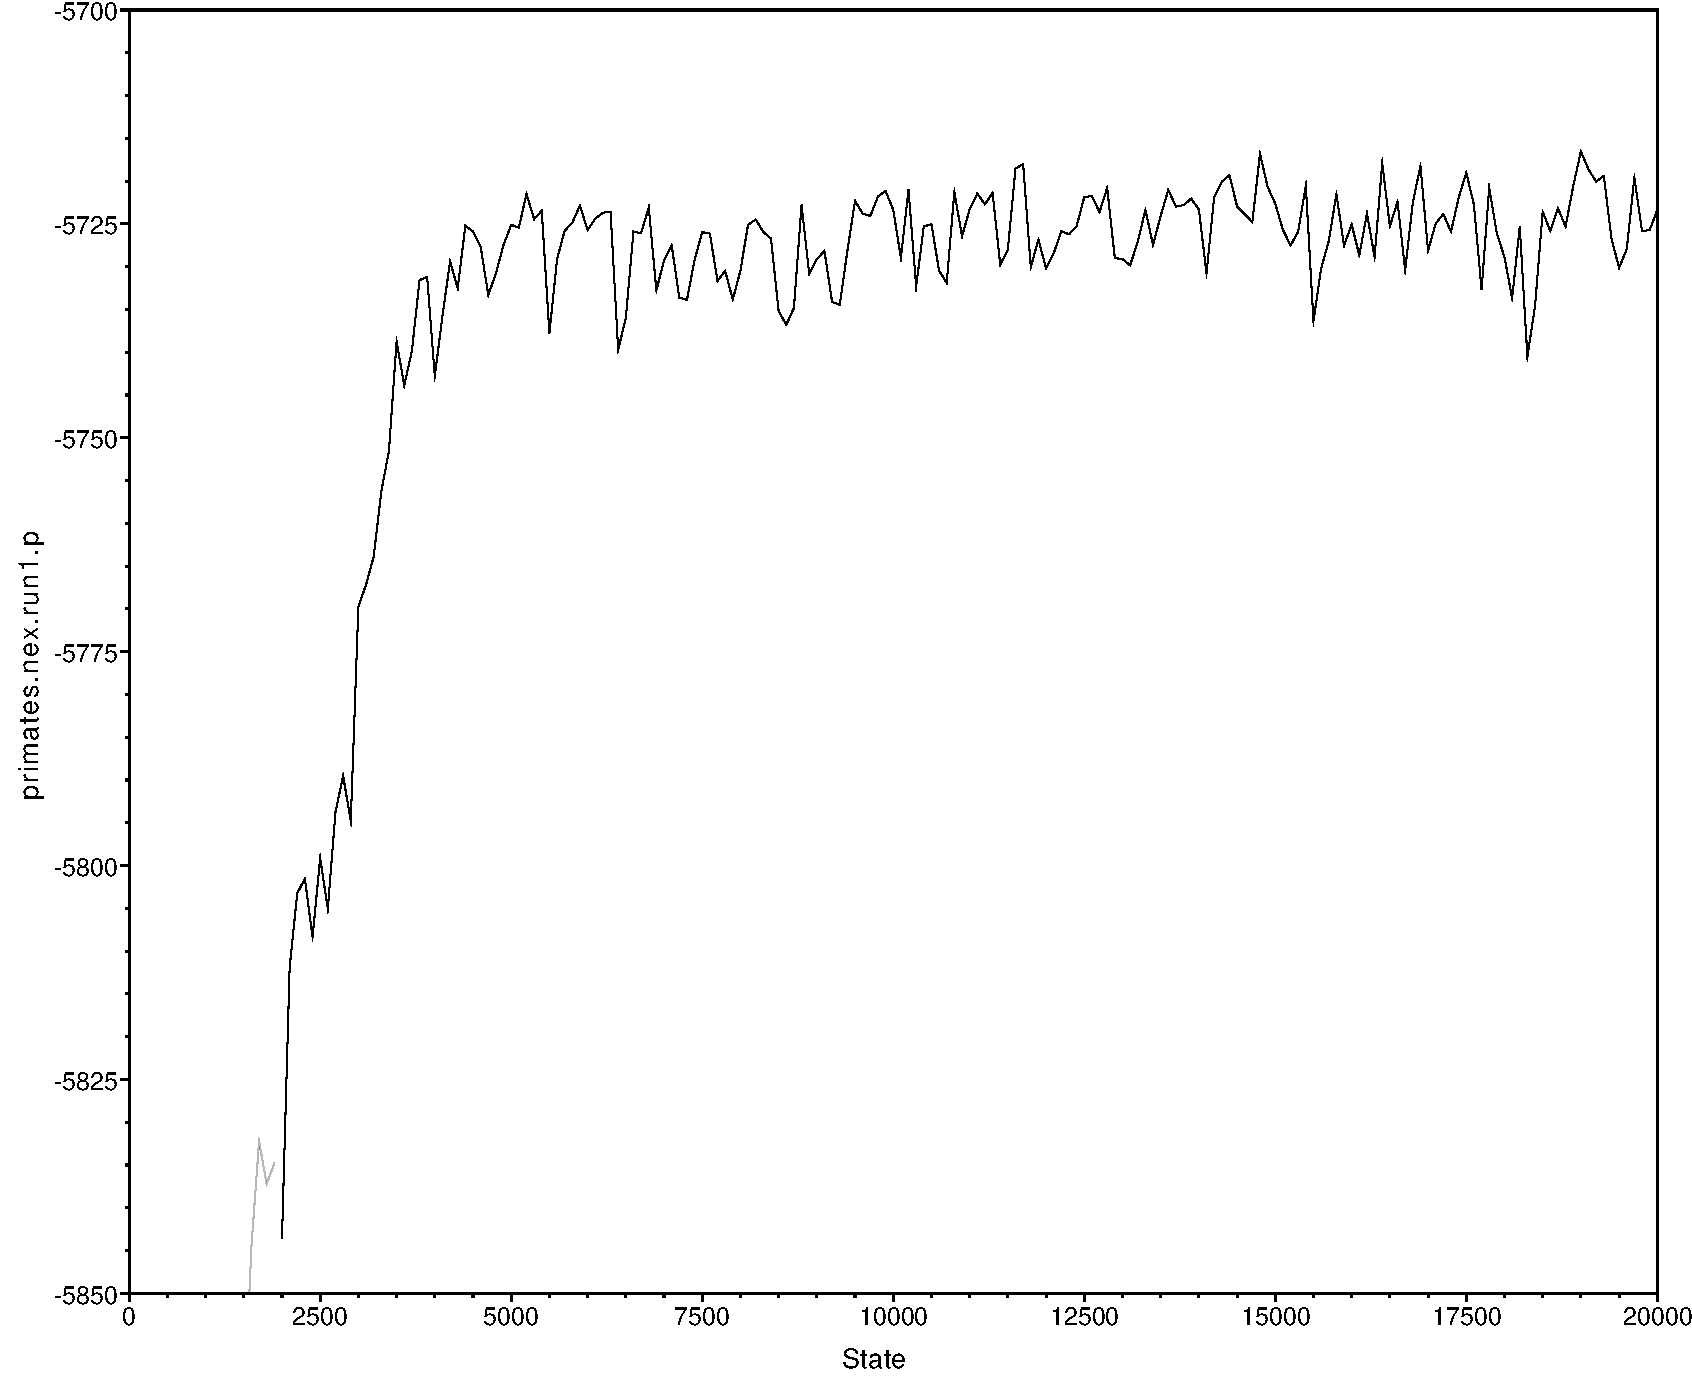
\includegraphics[width=0.5\textwidth]{trace.pdf}
\caption{Example trace plot. The plot suggests the burnin should probably be about 5000.}
\end{figure}

\item View the trace plots of all the parameters by selecting the parameter names in the
\texttt{Traces:} panel (lower left hand side of window). 
For example, transition rate for A-C are called \texttt{r(A<->C)}. 

\item If the MCMC has converged, the trace plots should look nice ``furry 
caterpillars'' such as Figure 2. 
Your MCMC analysis was much too short to produce furry caterpillars.

\item Another way to convergence diagnostic is the effective sample size (ESS) 
value of the trace. These are listed in the \texttt{Traces:} panel.
ESS values over 200 are considered adequate.

\item By default, Tracer discards the first 10\% of samples as \textit{burn-in}.
This is shown in the \texttt{Trace Files:} panel in the upper left side of the window.
The burn-in of an MCMC run is the initial part of a run where the MCMC
may have been stuck in a low probability region of parameter space.
For the trace in Figure 1, the burn-in should probably be 
adjusted to at least 5000.

\end{enumerate}

\begin{framed}
\noindent
\textbf{Question 2:} \\
By double-clicking on the \textit{Burn-In} value in the \texttt{Trace Files:} panel
modify the burn-in to a reasonable amount. 
How does this affect the ESS values? \\
\\
By repeating step 1 and 2 above, load the file \texttt{primates.nex.run2.p} 
from the second MrBayes run 
(remember MrBayes ran two parallel runs).
Set an appropriate burn-in for the second run,
and then click on \texttt{Combined} to view the samples from both MCMC runs combined.
How does this affect ESS values? \\
\\
You now have both ESS and ASDSF values. Do they agree on whether or not convergence has been reached? \\
\\
Send me a screen shot of your entire Tracer window with combined runs showing.
\end{framed}

\begin{figure}
\centering
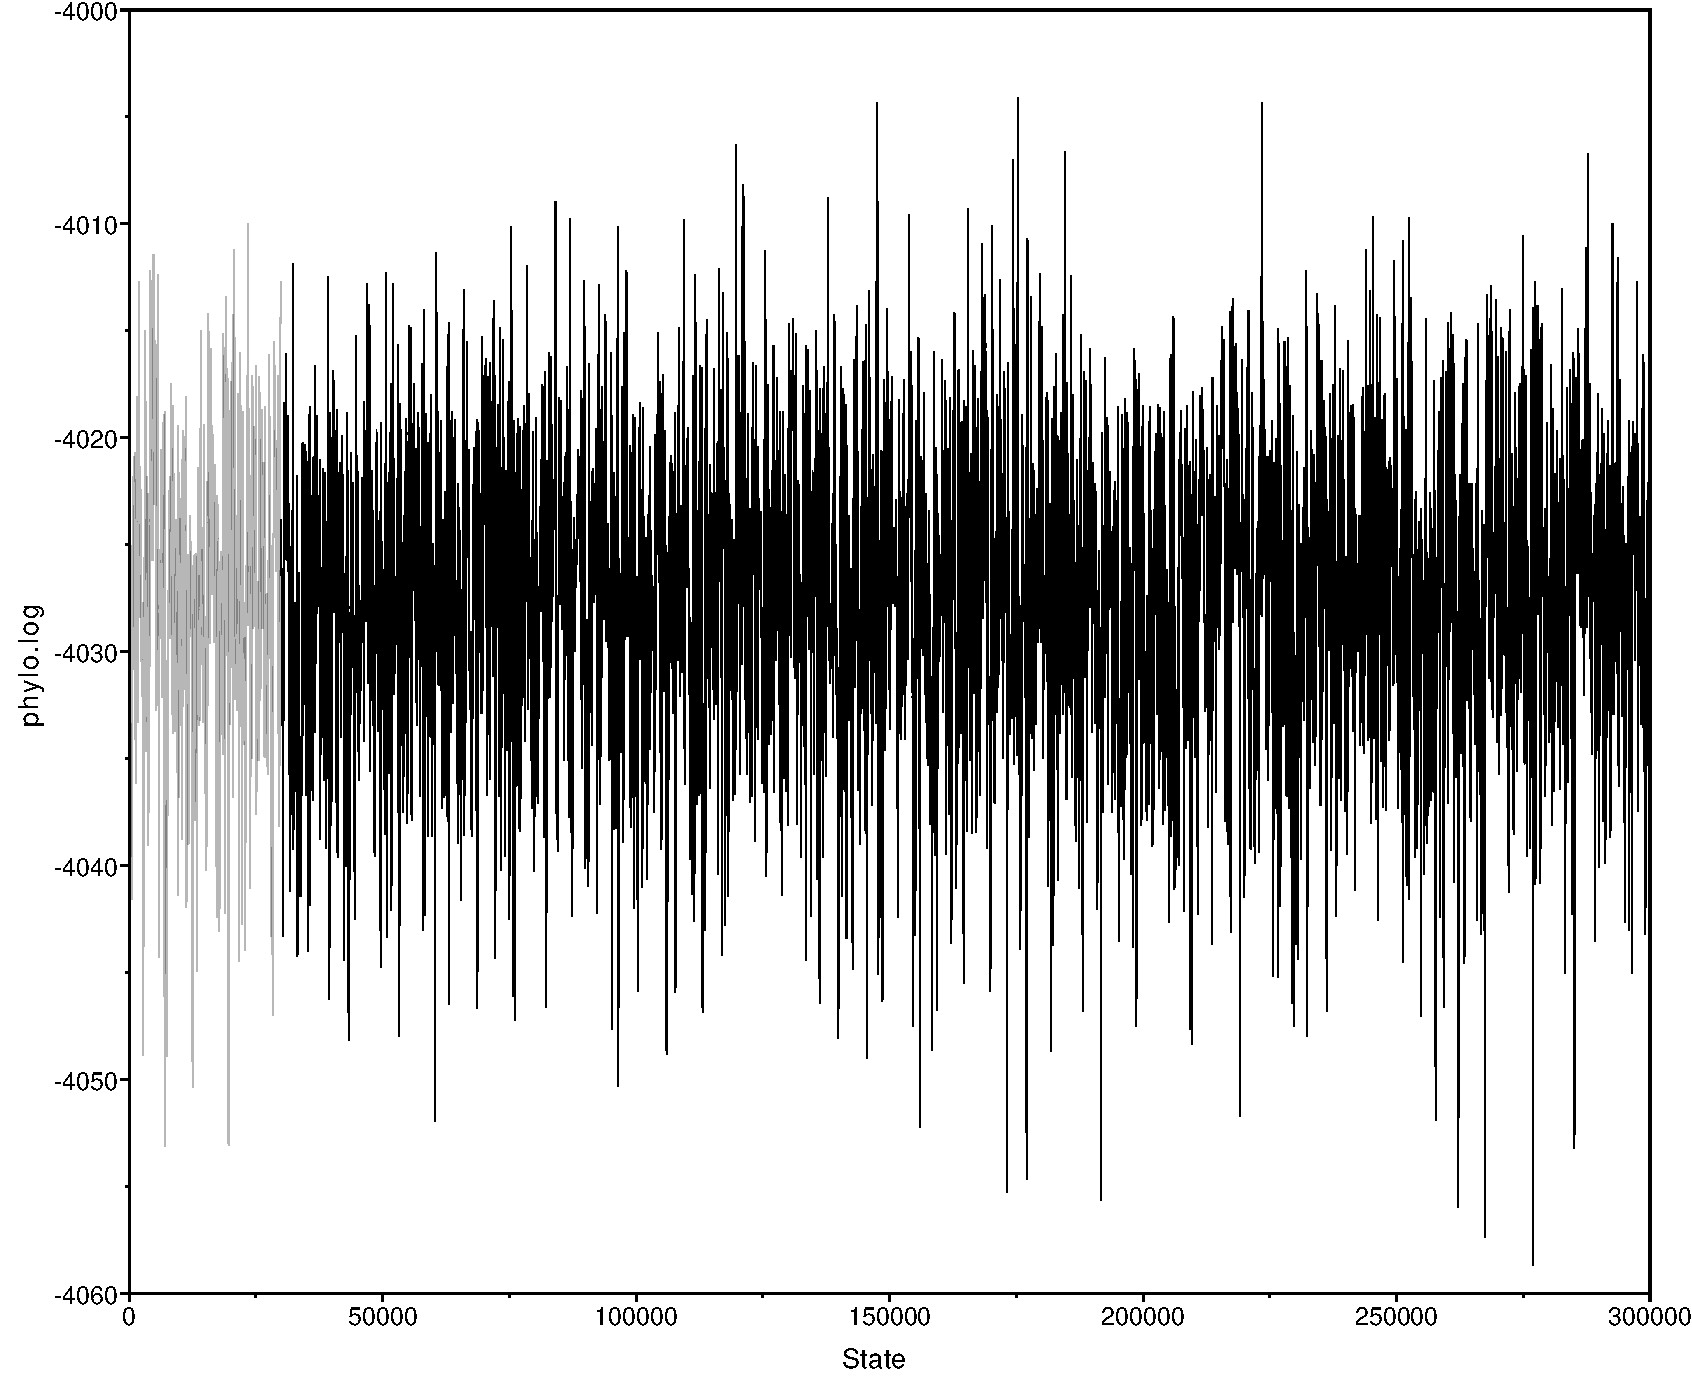
\includegraphics[width=0.5\textwidth]{log.pdf}
\caption{Example ``furry caterpillar'' trace plot for a nicely converged MCMC analysis.
This trace has an effective sample size (ESS) value of 2653.}
\end{figure}

\section{Bayesian Divergence Time Estimation using BEAST}

\textbf{BEAST} \citep{bouckaert2014beast} is probably the second most widely used Bayesian phylogenetic software,
and it became popular primarily because of the relaxed clock models
that were first implemented in BEAST.
Though all these models are now implemented in both MrBayes and BEAST,
we are going to do this exercise in BEAST since it has a very different user interface.

\subsection{Non-Bayesian Divergence Time Estimation}

There are a pair of non-Bayesian methods for estimating divergence times
implemented in the program \textbf{r8s} \citep{sanderson2003r8s}.
They are (1) a nonparametric rate smoothing approach, and (2) a
semiparametric penalized likelihood method that combines 
likelihood and the nonparametric rate smoothing penalty function.
These have been widely used in the past, but their use is (arguably) decreasing
with the advent of Bayesian approaches to fossil dating.

\begin{figure}
\centering
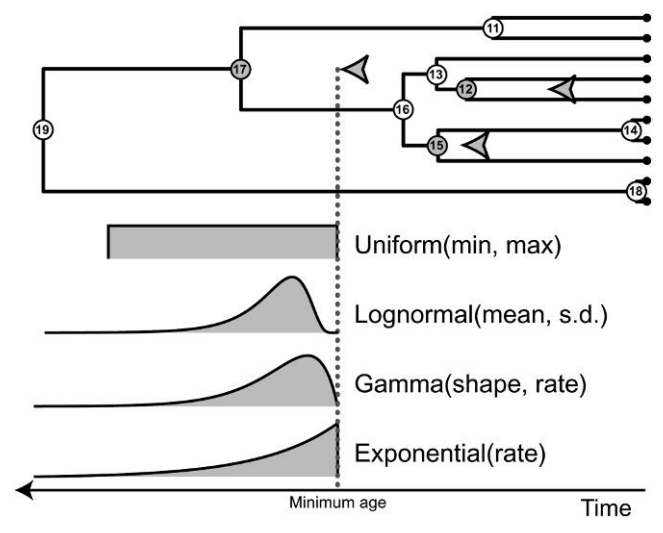
\includegraphics[width=0.5\textwidth]{node_calibration.png}
\caption{Four probability densities commonly used as priors on node ages,
shown here calibrating node 17. The grey dotted line
represents the minimum age constraint placed on the age of node 17 
by a fossil descendant (grey arrow).
Image from \protect\citet{heath2012hierarchical}.}
\end{figure}

\subsection{Tip-Dating Vs. Node-Dating}

In this lab we'll be covering the commonly used approach
called \textit{node-dating}, in which a fossil is assigned to an internal node
of the phylogeny, thus constraining the minimum age of the internal node.
A probability density is used as a prior for the calibrated node (see Figure 3).
This is problematic because the fossil may be misplaced in the phylogeny,
and the choice of a prior is usually arbitrary.

The \textit{tip-dating} (or total evidence)
approaches use morphological data from the fossil and extant taxa
to place the fossil just as if it was another tip.
The difficulty with this approach is that morphological
data is needed as well as molecular data.
Furthermore, models of morphological character evolution are
under developed.

Another approach, that can be used in conjunction
with either tip-dating or node-dating is the fossilized birth-death (FBD)
process \citep{heath2014fossilized}. This models speciation, extinction, and the fossil recovery rate
together. It can integrate over all possible placements for the
fossil taxon (including being a direct descendant) and so does
not require specifying an arbitrary prior for the node age.

Unfortunately we only have time to cover node-dating, but
you should look into these other approaches for your projects.

\subsection{Using BEAUti to Create an XML file}

BEAST uses eXtensible Markup Language (XML) files for initial input. 
These files allow for the combination of text and additional information. 
In this way the character matrix data can be stored alongside the analysis 
specifications that you will make for specific analyses. 
The XML file specifies sequences, node calibrations, models, priors, 
output file names, etc. 
We are starting with a NEXUS file with today's exercise, 
which we need to convert to an XML. 
The program \textbf{BEAUti} (Bayesian Evolutionary Analysis Utility) 
will do this for you and is automatically included when you download BEAST. 

\begin{enumerate}

\item First open up the BEAUti program, which will be located within your BEAST folder. 
Now import your NEXUS file. \texttt{File -- Import Alignment}. 
Select the \texttt{primates.nex} file. 

\item We'll now set up a node age prior on the human-chimpanzee common ancestor. 
Select the \texttt{Priors} tab. 
Click on the \texttt{+} button to add a new prior.

\item In the \texttt{Taxon set label:} box label this prior \texttt{human-chimp}.

\item Select \textit{Home\_sapiens} and \textit{Pan} and add them to the group
by clicking on the \texttt{>>} box. Click \texttt{OK}.

\item Select the Normal distribution. Click the little arrow to the left of
the \textit{human-chimp.prior} button.

\item Set the mean to 6 and sigma to 0.5. We will assume a normal distribution centered around 6 million years with a standard deviation of 0.5 million years. This will give a central 95\% range of about 5-7 My, which corresponds to the consensus estimate of the date of the most recent common ancestor of humans and chimps.

\item Set up a second calibration point for the group \texttt{HomiCerco}
which includes everything except \textit{Lemur}, \textit{Saimiri}, and \textit{Tarsius}.
Give this a normal distribution with 24+/- 0.5 million years.

\item Let's also set up a topological constraint to make sure our tree is rooted
correctly. Add another prior called \texttt{ingroup}, selecting all taxa except
the \textit{Lemur}. Constrain this to be monophyletic by clicking the \texttt{monophyletic}
checkbox.

\item Note the default tree prior is a \textit{Yule Model}. This is 
a stochastic process that models only speciation. Let's change it to
a slightly more realistic \textit{Birth Death Model} that includes extinction.

\item Click on the \texttt{Site Model} tab. By default the substitution model is 
set to Jukes Cantor. Change it to GTR.

\item Click on the \texttt{MCMC} tab. Change the \texttt{Chain Length} value
to 800,000.

\item Under the \texttt{File} menu, click \texttt{Save As} and save the XML file.

\item Start BEAST and select the XML file you just generated. Click \texttt{Run}.


\begin{framed}
\noindent
\textbf{Question 3:} \\
It should run pretty fast. Once it is complete, open the \texttt{.log}
file in Tracer. How do the ESS values look? Should the MCMC be run longer? \\
\\
What is the estimated mean age of the ingroup's most recent common ancestor?
% ~35.3
\end{framed}

\item Now let's summarize the posterior distribution of trees and get
the 95\% highest posterior density (HPD) ranges for node ages. Open the program
\textbf{TreeAnnotator} that came with BEAST.

\item Enter an appropriate \texttt{Burnin percentage}.

\item Choose \texttt{Mean heights} for \texttt{Node heights}. This sets the heights (ages) of each node in the tree to the mean height across the entire sample of trees for that clade.

\item For the \texttt{Input Tree File} select the \texttt{.trees} file that BEAST
generated.

\item Enter a name for your output summary tree file and click \texttt{Run}.

\end{enumerate}

\begin{framed}
\noindent
\textbf{Question 4:} \\
Open the summary tree in FigTree. Figure out how to add the 
95\% HPD node age ranges as node bars to the tree. 
Also add the posterior probabilities on the nodes of the tree.
Send me a screen shot.
\end{framed}

\begin{framed}
\noindent
\textbf{Please email me the following:}
\begin{enumerate}
  \item The answers to questions 1-4.
  \item Screenshots for questions 2 and 4.
\end{enumerate}
\end{framed}

\bibliographystyle{plainnat}
\bibliography{\jobname} 

\end{document}

